% XeLaTeX can use any Mac OS X font. See the setromanfont command below.
% Input to XeLaTeX is full Unicode, so Unicode characters can be typed directly into the source.

% The next lines tell TeXShop to typeset with xelatex, and to open and save the source with Unicode encoding.

%!TEX TS-program = xelatex
%!TEX encoding = UTF-8 Unicode

\documentclass[11pt]{article}
\usepackage{geometry}                % See geometry.pdf to learn the layout options. There are lots.
\geometry{a4paper,left=2.5cm,right=3.5cm}                   % ... or a4paper or a5paper or ... 
%\geometry{landscape}                % Activate for for rotated page geometry
%\usepackage[parfill]{parskip}    % Activate to begin paragraphs with an empty line rather than an indent
\usepackage{graphicx}
\usepackage{amssymb}
\usepackage[english]{babel}
\usepackage{hyperref}

% Will Robertson's fontspec.sty can be used to simplify font choices.
% To experiment, open /Applications/Font Book to examine the fonts provided on Mac OS X,
% and change "Hoefler Text" to any of these choices.

\usepackage[protrusion=true]{microtype}
\microtypecontext{spacing=nonfrench}

\usepackage{fontspec,xltxtra,xunicode}
\defaultfontfeatures{Mapping=tex-text}
\setromanfont[Mapping=tex-text]{Verlag Extra Light}
\setsansfont[Scale=MatchLowercase,Mapping=tex-text]{Helvetica Neue}
\setmonofont[Scale=MatchLowercase]{Anonymous Pro}


\title{\vspace*{-1\baselineskip}Portfolio}
\author{Åsmund Ødegård \\ @mandus \\ \url{https://github.com/mandus}}\author{Åsmund Ødegård \\ @mandus \\ \url{https://github.com/mandus}}
\date{}                                           % Activate to display a given date or no date

\begin{document}
\fontsize{11}{15}\selectfont
\maketitle
\thispagestyle{empty}

\begin{minipage}[b]{0.45\textwidth}
Most of what I do end up as server-side code not suitable for inclusion in a visual portfolio. Also, I shall not claim that front-end design is my speciality. Nevertheless, in several projects and in particular those where the staffing is limited, it is required to work as a full-stack developer---all they way from the database and server-side logic to the user experience.
\end{minipage}
\hfill\rule[-1.7cm]{0.2pt}{5.7cm}\hfill
\begin{minipage}[m]{0.45\textwidth}
The purpose of this document is thus to showcase some projects where I have been involved in front-end work (and where I legally am allowed to use images for this purpose). Only rarely will my work be on publicly available pages, so it is easier to showcase the sites in a document rather than pointing to the web-pages. 
\end{minipage}

\vspace{2cm}
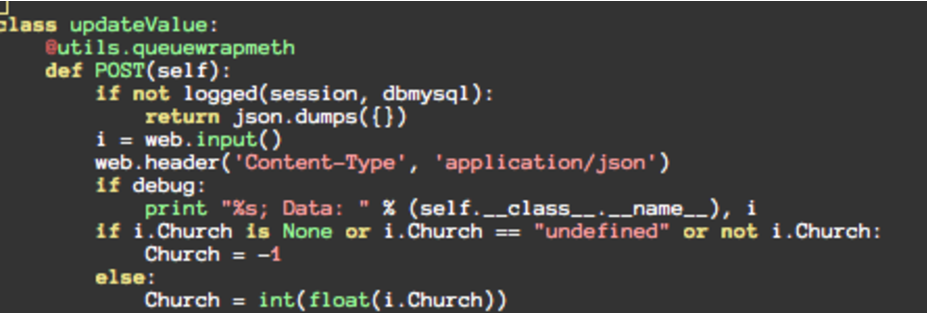
\includegraphics[scale=0.8]{portfolio-graphics/py-code.pdf}

\vspace{-3cm}
\hfill
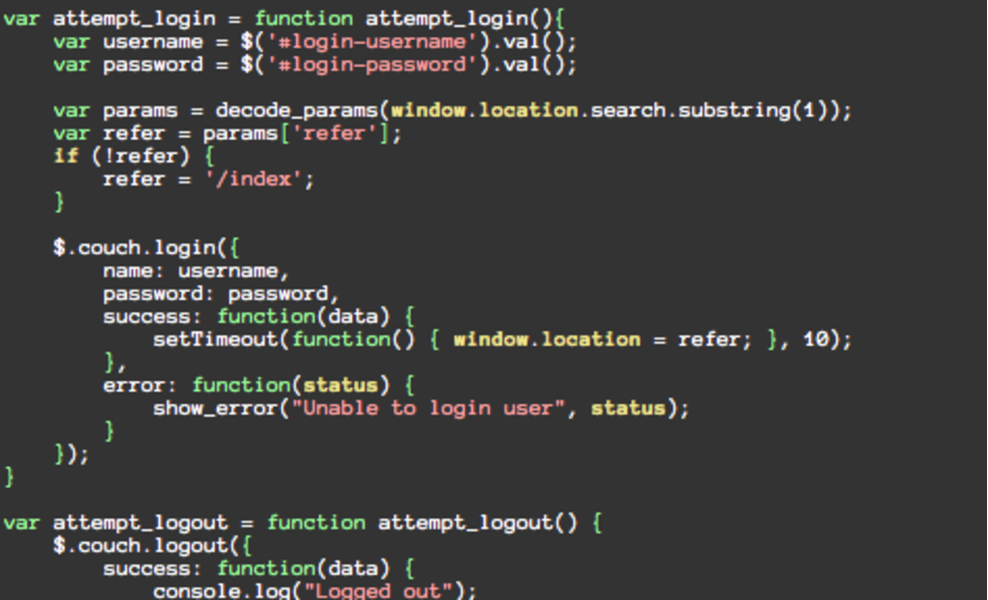
\includegraphics[scale=0.7]{portfolio-graphics/js-code.pdf}

\section*{SmartBlikk}
SmartBlikk is implemented in PHP using the Slim micro-framework and Twig template engine. On the front-end we utilise the Bootstrap and jQuery frameworks together with custom Javascript code. At the stage of these images the product is still unfinished, but I show a few images from the wizard for building custom reports, and a view of administrative settings for APIs. 

Some of the surrounding graphics in these images (mainly the header/footer in the first image) were already set up when I started working on the project. However, the main content on these pages, with the accompanying back-end functionality, has been implemented by me. 

\vspace{2\baselineskip}
\noindent
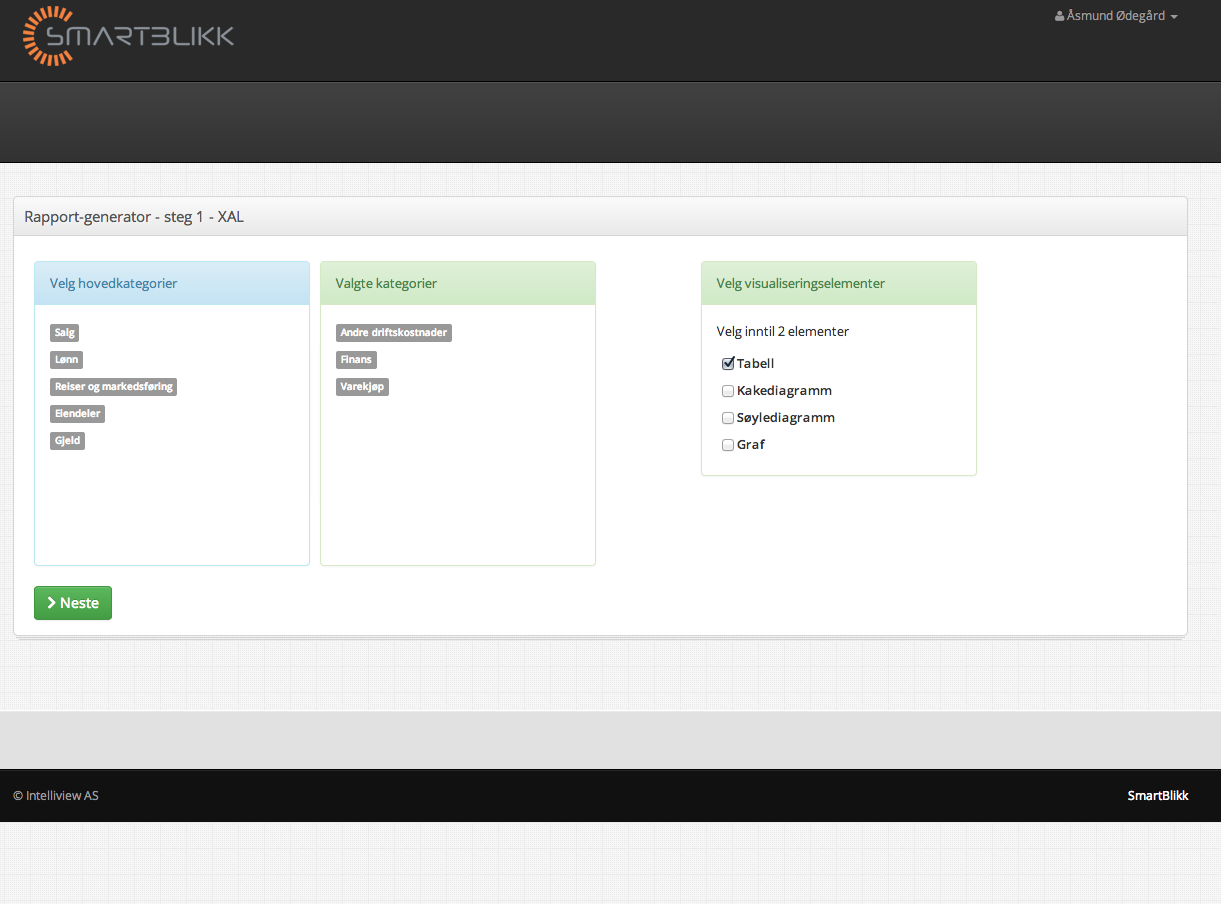
\includegraphics[width=\textwidth]{portfolio-graphics/sb-stage1.png}

\vspace{\baselineskip}
\noindent
The user can move categories between the boxes on the left side in order to enable or disable main categories in the report. In addition a few visuals to be used in the report can be selected already at the first stage. These visuals will then be live updated in subsequent steps as further choices is done for the report.
 
\noindent
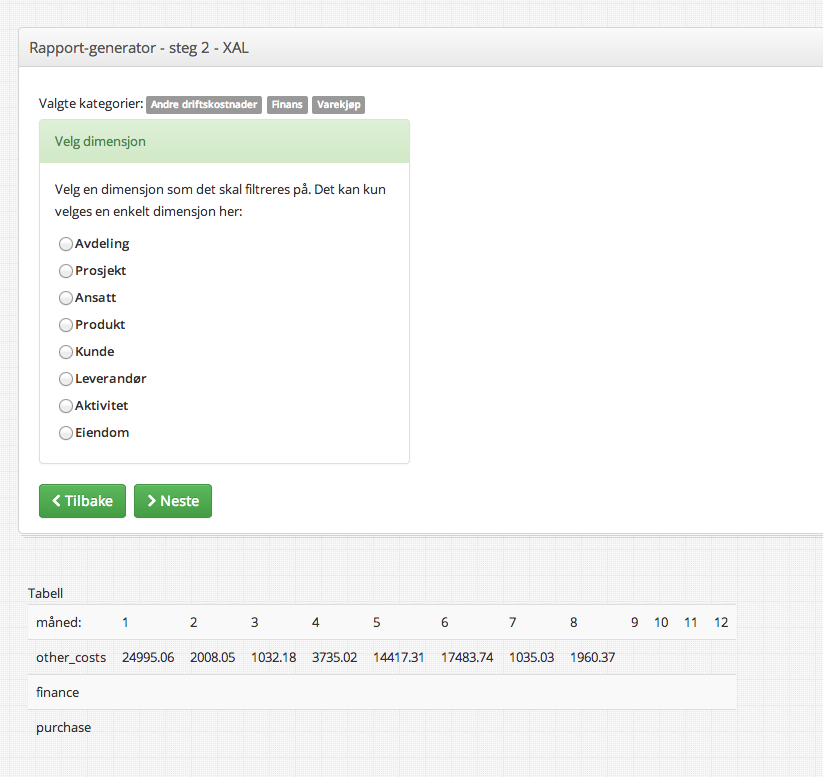
\includegraphics[width=\textwidth]{portfolio-graphics/sb-stage2.png}

\vspace{\baselineskip}
\noindent
On the next stage in the wizard, the used can further customise the report by selecting dimensions. Ajax is used to fill the selected visual (in this case table) such that the user-interface remains responsive, and the data is updated as choices is done in the list of radio-buttons.

\noindent
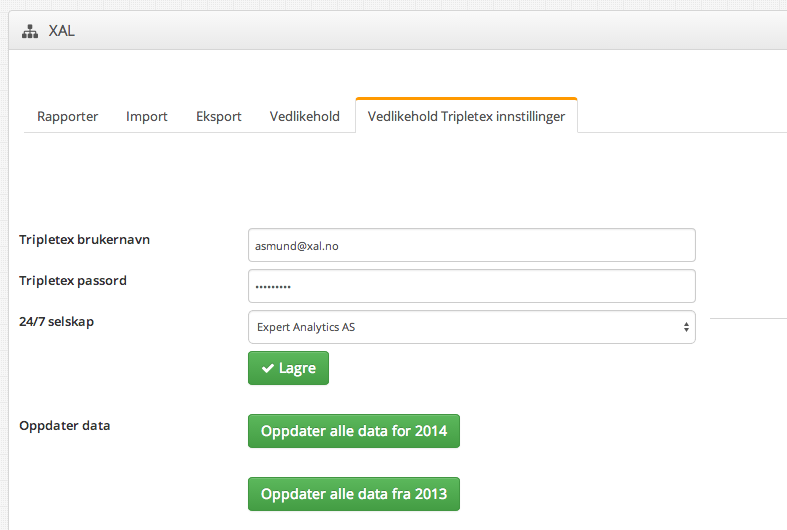
\includegraphics[width=\textwidth]{portfolio-graphics/api-maint.png}

\vspace{\baselineskip}
\noindent
On this screen, the user will be able to maintain settings for one of the implemented API integrations. The buttons at the bottom will trigger calls to the backend server that rebuilds the internal dataset. Again we are using ajax-calls for this such that the user interface remains responsive. In case the user stays on this page, a message will appear when the task is finished, mentioning some statistics for the imported data. As a side-note, the user credentials dialog work together with the security functions on the backend. We do not want to store password in cleartext in the database, so the cleartext password will only be available in memory. As SmartBlikk needs to know the password when making calls to the API on the user's behalf, we utilise a symmetric AES algorithm for the encryption.  

\section*{GitterApp}
For a Norwegian SME producing physical security items for the business sector, we have created a web-based system for configuration of security grilles. The application is implemented using CouchDB as back-end and HTML5 front-end utilising jQuery and custom Javascript code. The visual appearance is based on the Bootstrap framework. This application is somewhat unique in that there is no application server involved except the database server; the sources are served directly from the CouchDB server and all processing are done on the front-end. The system is running in the ``cloud,'' on an Amazon EC2 instance. 

I display three pages from this system; the log-on screen presented when you enter the site, and excerpts from two different administrative pages. I am not able to showcase the main part of the system where our customer configure the grilles, but the main features of that system is live calculation of the final price and validation of completeness; i.e. there are certain features that must be selected in order to ensure a complete security grille. There are about 20 different settings, many of them with several different options, which yields a fairly complex system. 

GitterApp was fully designed and implemented by Expert Analytics. I have implemented everything on display here, while Ola Skavhaug implemented some other parts of the system.

\vspace{2\baselineskip}
\noindent
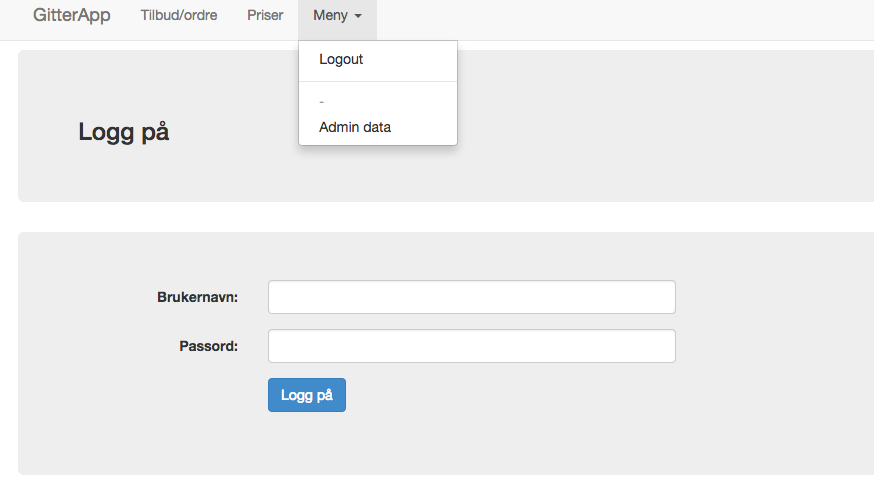
\includegraphics[width=\textwidth]{portfolio-graphics/GA-1.png}    
The system is implemented in a lean and simplistic style, featuring only three main pages, and with some administrative features only accessible by super-users.

\vspace{2\baselineskip}
\noindent
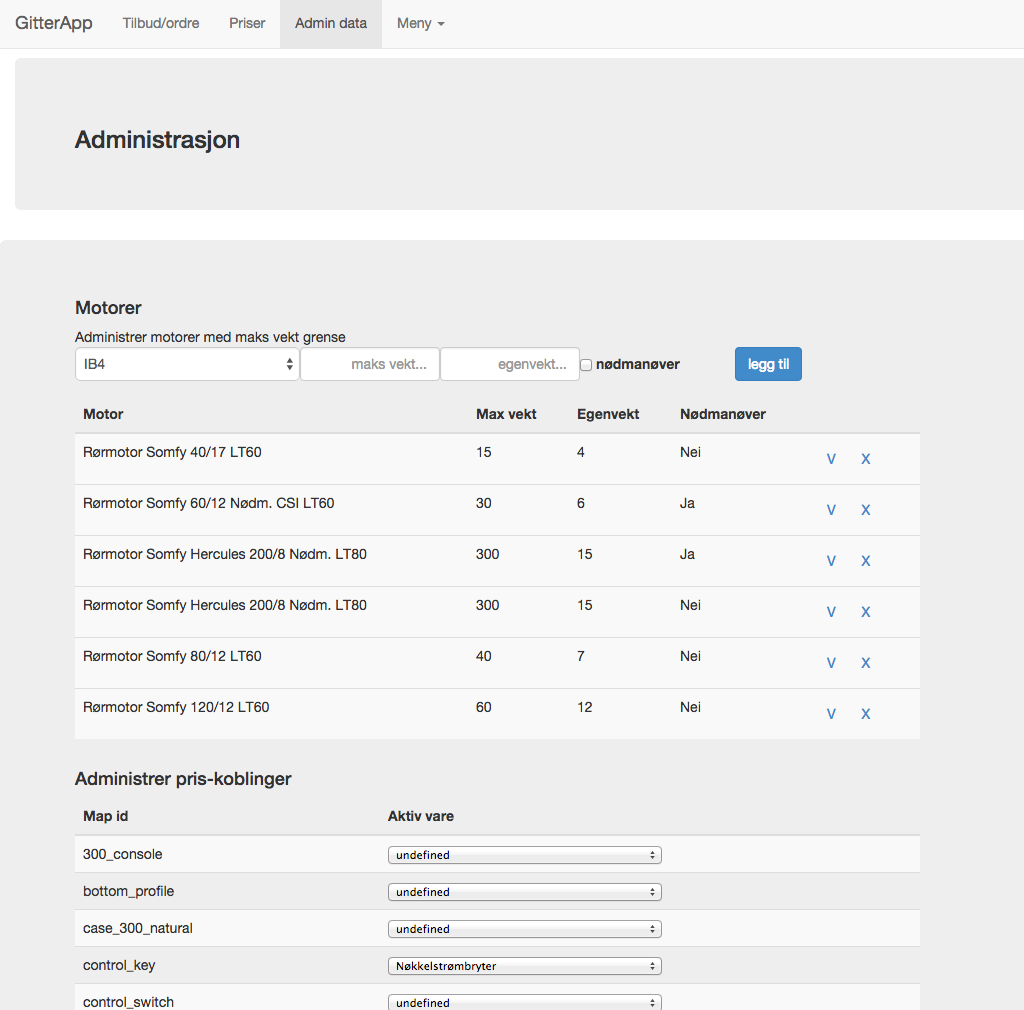
\includegraphics[width=\textwidth]{portfolio-graphics/GA-2.png}    

\vspace{2\baselineskip}
\noindent
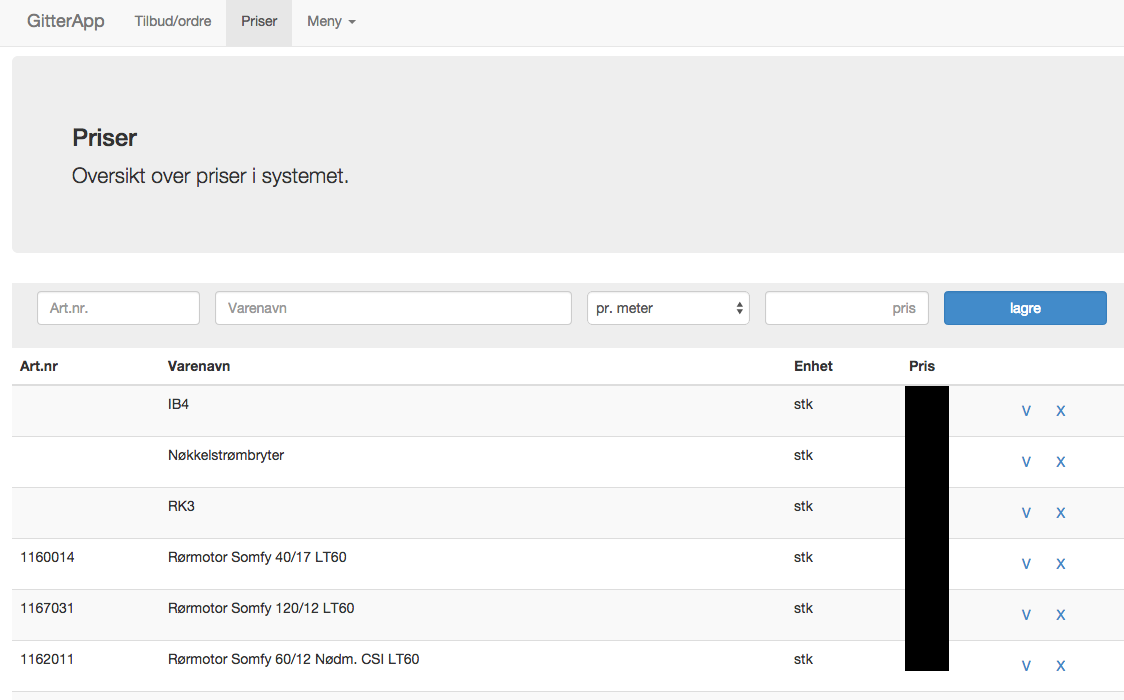
\includegraphics[width=\textwidth]{portfolio-graphics/GA-3.png}    

\section*{Web.py Project}
Finally, I will show some images from a project implemented using the Python Web.py framework and a WSGI application server. Due to the nature of this project, I must edit out the details. The system was implemented for an volunteer-based non-profit international organisation. As for the other projects, Bootstrap, jQuery and custom Javascript is used on the front-end. There are a lot of calculations going on in the front-end when users utilise this tool for their analysis, with ajax-based interaction with the python application server when necessary. The Highchart Javascript library is used to generate live dynamic graphs in the browser. 

I was the sole programmer on this project, but worked together with a designer/UX-specialist who organised the information into tabs and worked on placement of the elements. This was crucial for the project since it was to be used by several persons with quite different prior competences. We both need to implement a natural path through the wizard, as well as providing some flexibility for more advanced users.

\vspace{2\baselineskip}
\noindent
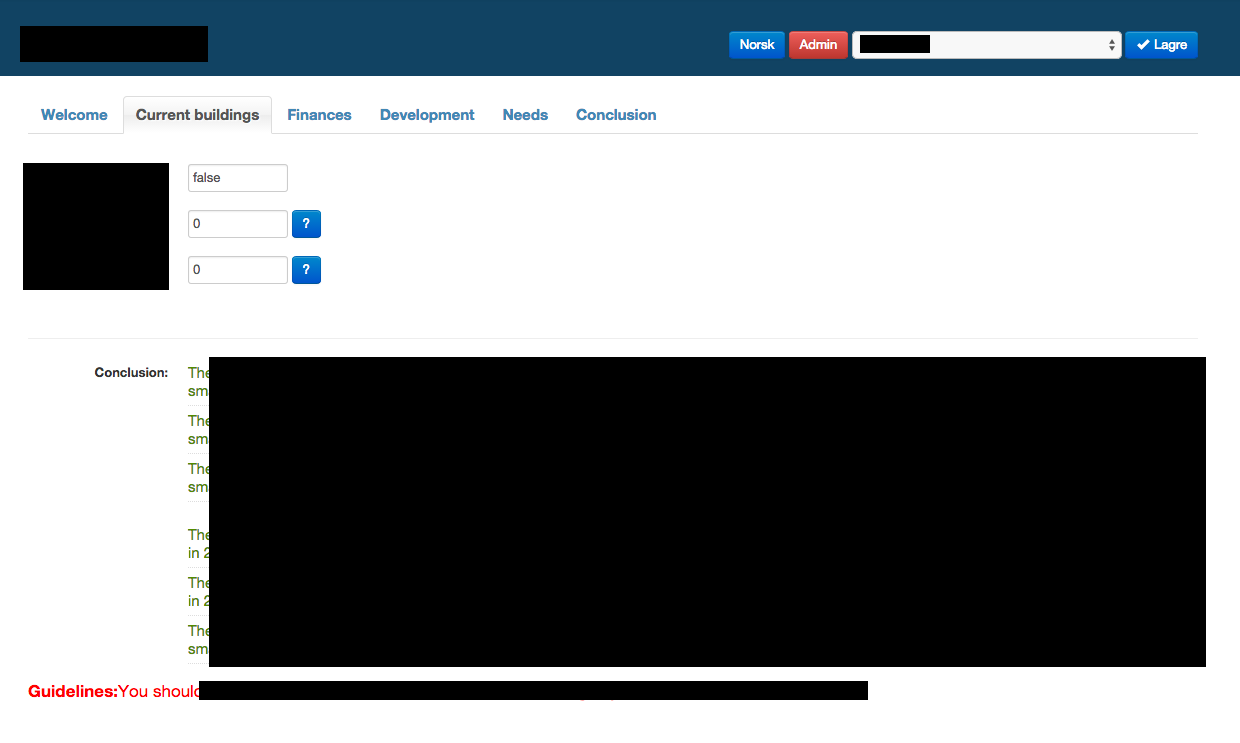
\includegraphics[width=\textwidth]{portfolio-graphics/GH-1.png}    

\vspace{2\baselineskip}
\noindent
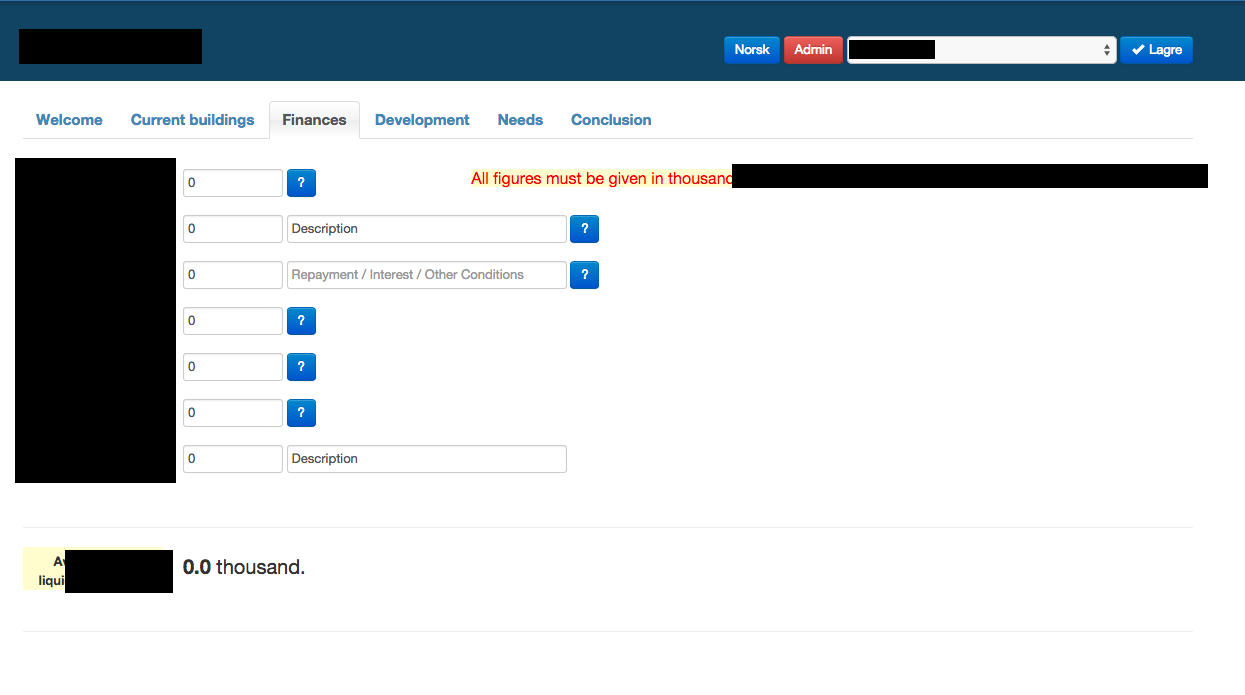
\includegraphics[width=\textwidth]{portfolio-graphics/GH-2.png}    

\vspace{2\baselineskip}
\noindent
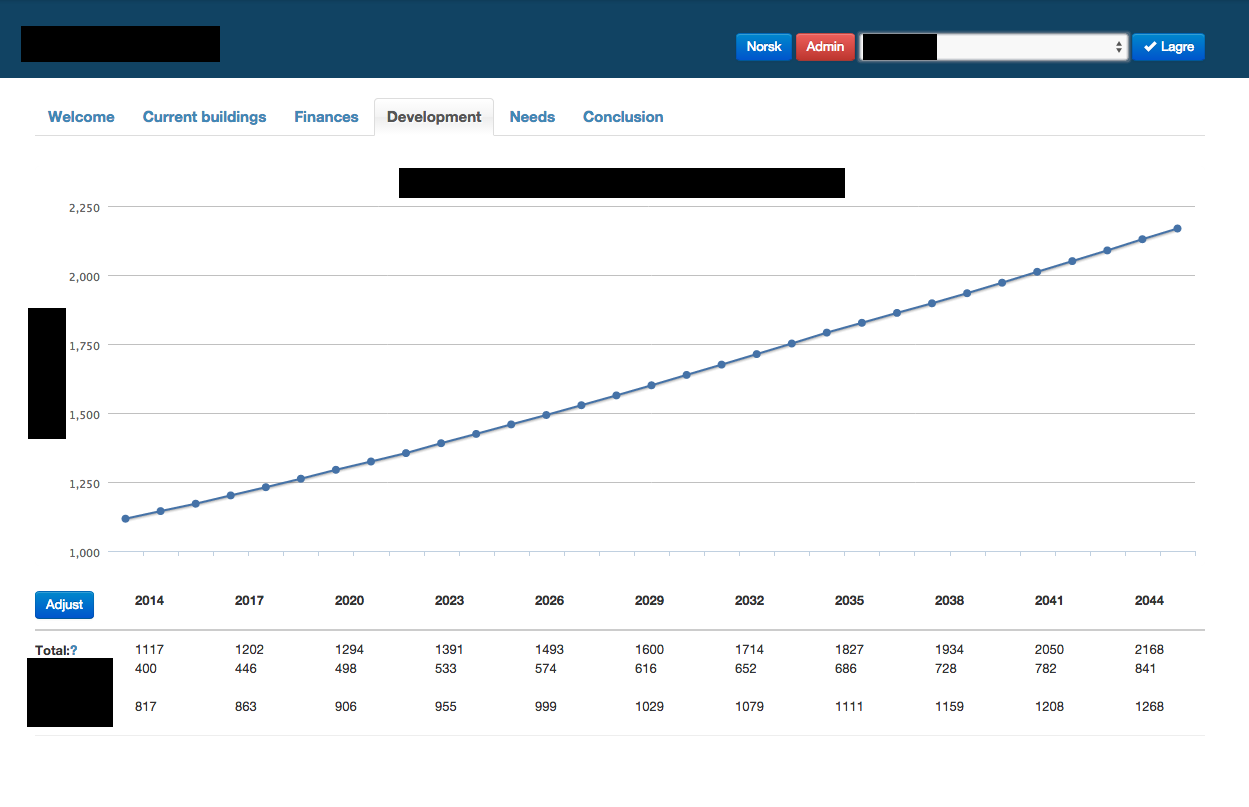
\includegraphics[width=\textwidth]{portfolio-graphics/GH-3.png}    

\vspace{\baselineskip}
\noindent
This is actually the most important and advanced part of this system. Based on some data made available by the organisation, algorithms are used to compute a forecast graph for the next 30 years, as well as key accompanying numbers included in the table below. Using the ``Adjust'' button, the user may modify some parameters for the algorithm which will trigger recalculation of the forecast. When the updated forecast is finished, it will be loaded back in the graph. There is a lot of stuff going on both in Javascript on the client side and on the back-end application server, which is all hidden for the user. The user may even visit some of the other sub-pages while the calculations are carried out, if they want.

\section*{Conclusion}
Hopefully these images provide some ideas on what Expert Analytics will be able to deliver in terms of front-end work, given that this is not our main area of expertise. Unfortunately I do not have a lot of recent code publicly available, but the PySE code that was an important part of my PhD work is available at \url{http://sourceforge.net/projects/pyfdm/}. Recently this code was cloned by another researcher and made available at \url{https://bitbucket.org/sinayoko/pyse}; the original code may be easier to browser there but note that the researcher who uploaded the code has made a few updates. When looking at PySE as a reference, please keep in mind that this code about ten years old now, so both my coding-style and the community at large have evolved quite a bit since then.
 
\end{document}  
